% 导言区
\documentclass[UTF8,12pt]{ctexart}   % 中文文章类
\usepackage{amsmath}                 % 公式
\usepackage{graphicx}                % 插图
\usepackage[backend=biber,style=gb7714-2015]{biblatex} % 国标参考文献
\addbibresource{ref.bib}             % 数据库

\title{基于深度学习的图像去噪研究}
\author{张小明 \\ \small 中国科学院自动化研究所}
\date{\today}

\begin{document}
	\maketitle
	
	\begin{abstract}
		本文提出一种……(中文摘要)
	\end{abstract}
	
	\begin{abstract}[en]   % 英文摘要
		This paper proposes …
	\end{abstract}
	
	\section{引言}
	研究背景如图~\ref{fig:lenna} 所示。
	
	\begin{figure}[ht]
		\centering
		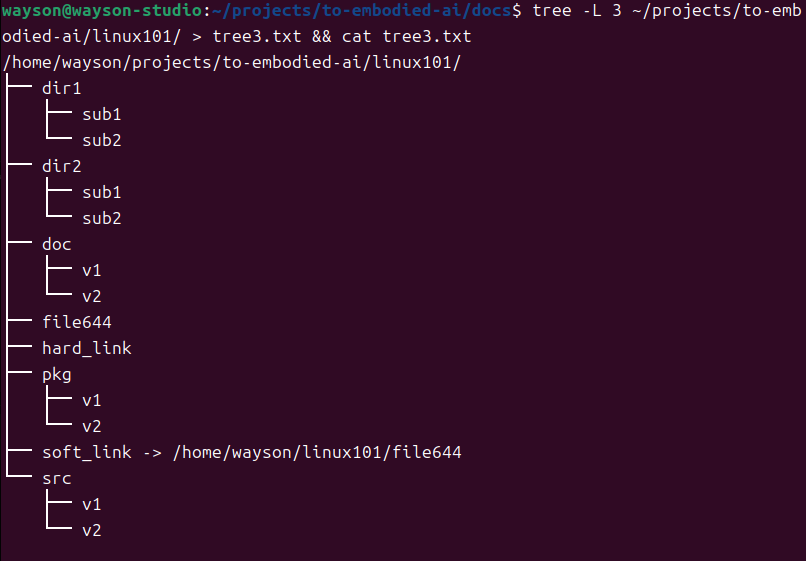
\includegraphics[width=0.4\linewidth]{lenna.png}
		\caption{测试图像}
		\label{fig:lenna}
	\end{figure}
	
	\section{方法}
	信噪比定义为
	\begin{equation}
		\mathrm{PSNR}=10\log_{10}\frac{255^2}{\mathrm{MSE}}.
	\end{equation}
	
	\section{实验}
	结果见表~\ref{tab:result}。
	
	\begin{table}[ht]
		\centering
		\caption{PSNR 对比}
		\begin{tabular}{cc}
			\hline
			方法 & PSNR/dB \\
			\hline
			传统 & 28.3 \\
			本文 & \textbf{32.1} \\
			\hline
		\end{tabular}
		\label{tab:result}
	\end{table}
	
	\printbibliography
\end{document}